\documentclass[11pt]{article}
\usepackage{graphicx}
\usepackage{float}
\usepackage{mathtools}
\newcommand\given[1][]{\:#1\vert\:}

\title{Second Homework: Causal Inference}
\author{Francesco Saverio Zuppichini}
\begin{document}
\maketitle
\section{Structure of the network}
My model represents weightlifting.  

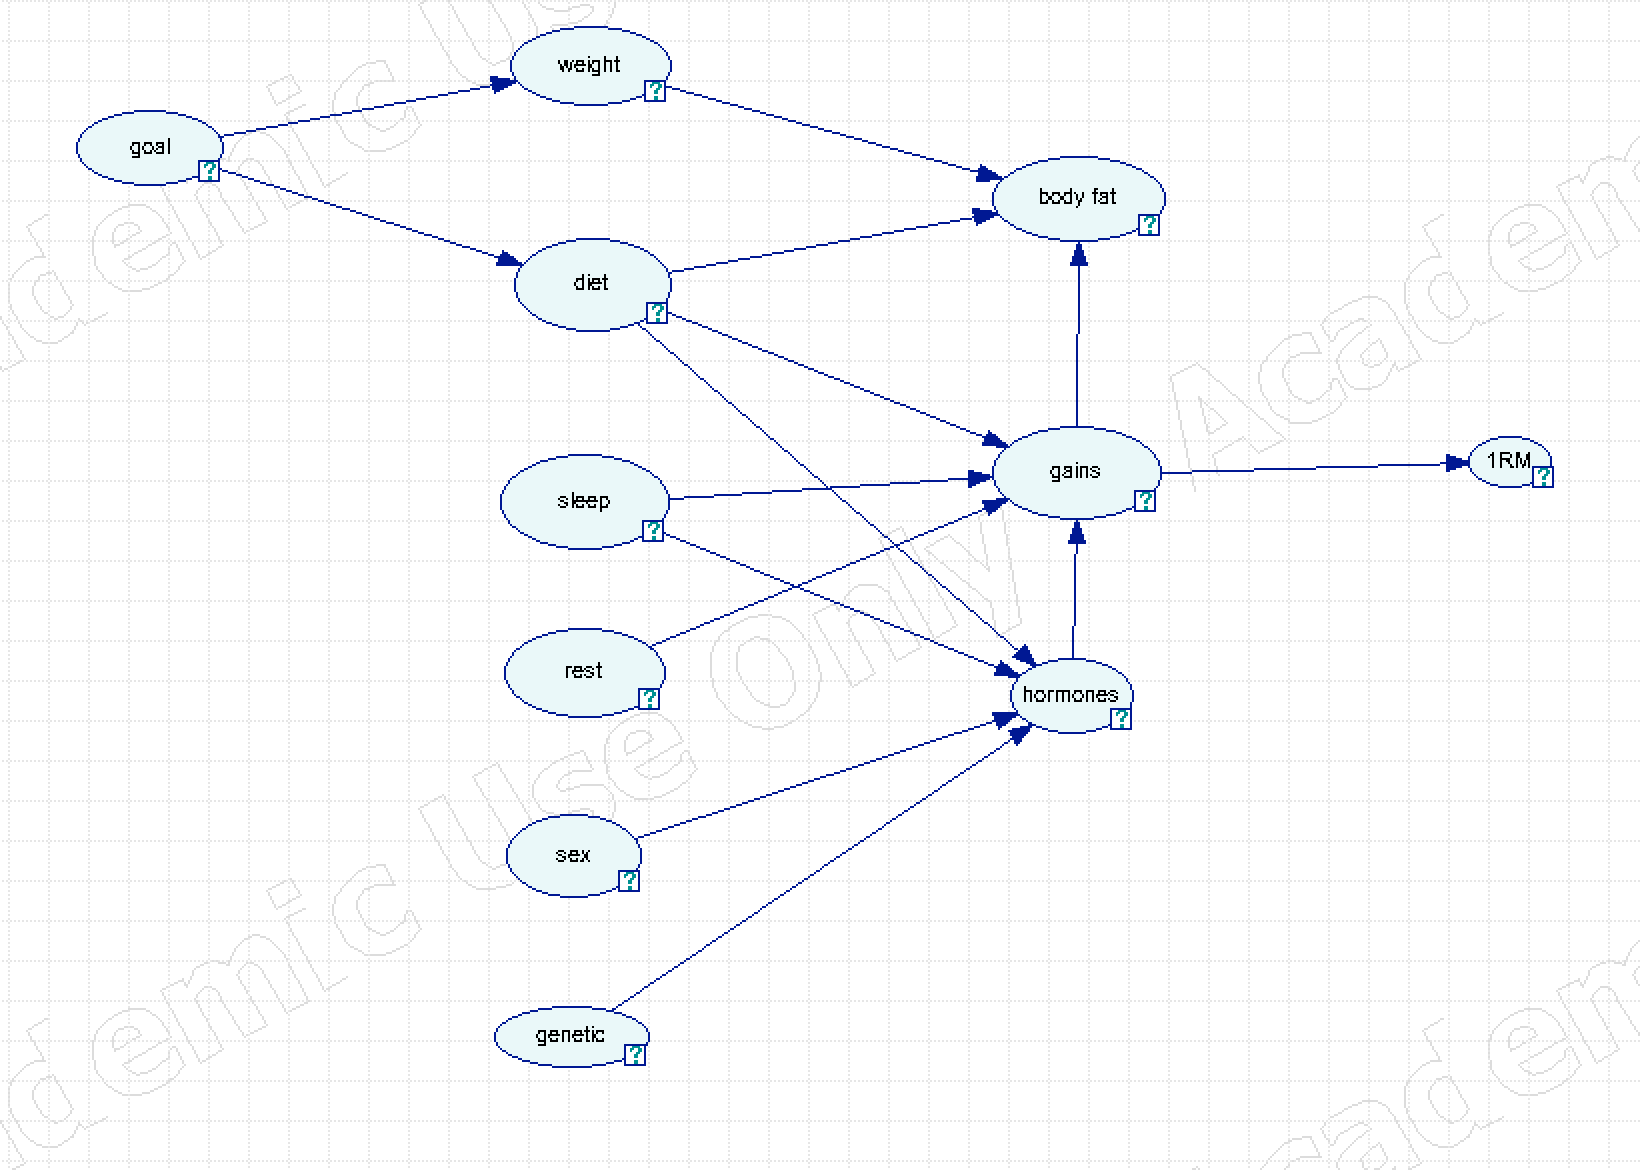
\includegraphics[width=\textwidth]{./images/net.png}

The variables are eleven in total. In the program, I renamed the state
name for better readability. It follows a description of each variable
in order of apperance from left to right.

\begin{itemize}
\item
  goal. The final goal of the athlete. It can be bulking, gain muscle, or
  cut, loose body fat. States are bulk and cut
\item
  weight. If true, the athlete gains weight from last month, if false
  otherwise. The states are called increased and not\_increased
\item
  diet. Represent what the athlete eats. It's outcome is true, athlete
  eats around 200\textasciitilde{}400 kcal more that his baseline, false
  otherwise. These states are called surplus and defict
\item
  sleep. How much the athlete sleeps. We assume that sleep time begin
  around 23:00 \textasciitilde{} 00:00. The outcome is 1 if the athlete
  sleeps more that 7.5 hours, 0 otherwise.
\item
  rest. The hours between two workouts. enough if more than 36 hours,
  low otherwise.
\item
  sex. male and female.
\item
  body fat. increased and not\_increased from last month.
\item
  genetic. good or average. The genetic of the athlete.
\item
  hormones. low is hormone production is under average, high if more.
  Hormones such as gh and testosterone are essential to gains.
\item
  gains. Measured in grams of muscle per month. increase if more than
  300g, same otherwise.
\item
  1RM\_increase. In \% how much we increase the one range of motion from
  last month on the base exercises: deadlift, squat and bench press.
  increase if 5\% more than last month, not increase otherwise.
\end{itemize}

It follows an explanation of the arcs in the graph. body fat depends by
the weight, the diet, booth depend of the age, and the gains. The more
you gain the more you weight.

gains is the most important node. It depends by weight, diet, sleep,
rest and hormone production. The late, directly depend on sex, sleep and
diet.

1RM increase depends on the gains.

\subsection{State which is the objective of the network: for instance, highlight a couple of situations in which decision making could be difficult and in which the graph could provide valuable indications}

Probably a mix of situations for \textbf{gains}. For instance, if the athlete sleeps more than 7.5 hours, eat enough but does not rest more than 36 hours. An other could be where the diet prevents a correct hormones production but the athlete trains, sleep and rest well.

\subsection{Explaining how you decide the arcs orientation, in case they are not self- explaining}

They are all streigthforward.

\subsection{Which arrows can be reversed without being detectable by a statistical test? Explain why}

The following set of edges can be reversed without being detectable by a statistical test.
$(e(goal, weight), e(goal, diet), e(gains, 1RM increase))$


\subsection{Identify at least 4 couple of nodes (the node of each couple should be not directly linked to each other) and analyze their d-separation properties possibly conditioning on others}

The nodes of the net are denominated by the first two consonant in the name for simplicity.
\begin{enumerate}
	\item (\textbf{goal}, \textbf{body\_fat})
These are the paths: $\{GL,WT,BF\}, \{GL,DT,BF\}, \{GL,DT,GN,BF\}, \{GL,DT,HR,GN, BF\}$

\item (\textbf{goal}, \textbf{gains})
These are the paths: $\{GL,DT,GN\}, \{GL, WT, BF, GN\}, \{GL,DT, BF, GN\}  \{GL, DT ,HR, GN\}, \{GL, WT, BF, DT, GN \}, \{GL, WT, BF, DT, HR, GN \}$


$BF$ is a collider for $WT, DT, GN$ so it already blocks some paths. We can condition on $DT$ to block al pat
\item (\textbf{goal}, \textbf{hormones})
These are the paths : $\{GL, WT, BF, GN, HR \}, \{GL, WT, BF, DT, HR \}, \{GL, WT, BF, DT, GN, HR \}, \{GL, DT, BT, GN, HR \}, \{GL, DT, GN, HR \} \{GL, DT, HR \}$.

As before, we can block on $DT$ to block all paths between $GL$ and $HR$.

\item (\textbf{diet}, \textbf{sleep})
These are the paths: $\{DT, GN, SL \}, \{DT, BF, GN, SL \}, \{DT, HR, GN, SL \}, \{DT, GL , WT, BF, GN, SL \},  \{DT, GL , WT, BF, GN, HR, SL \}$

All the paths are already blocked by $GN$ that is a collider.
\end{enumerate}

\subsection{Discuss how d-connected variables are in fact dependent in the real problem, while d-separated variables are instead independent in the real problem.}

\begin{itemize}
\item
  \texttt{goal} and \texttt{weight} are dependet since the goal that we
  choose determinate the weight we want to have
\item
  \texttt{goal} and \texttt{diet} are dependent since the goal we picked
  also must be followed by a correct diet. If we want to loose weight,
  we must eat less
\item
  \texttt{diet} and \texttt{sleep}. They independent, since what a
  person eat does not have repercussion on the sleep time an quality.
\item
  \texttt{hormones} and \texttt{body\ fat} are likely dependent since if
  an athlete produces more hormones it can gains more muscle and increase
  his body fat. Unfortunally, it is scientific prooved that is
  impossibile to gain muscle and loose fat at the same time. For the
  interested reader it follows a very simple explanation. To syntetize
  new muscle tissue the body needs to have a surplos of energy. Thus we
  must eat more than our base metabolism needs, this is called
  `bulking'. Having more energy leads to gain more weight and some body
  fat. The amount of body fat is directly proportional at the amount of
  kcal in surplus. Hoewer, they are several factors that also can
  influence the amount of body fat in a person, such as a history of bad
  diet and poor training.
\item
  \texttt{gains} and \texttt{body\ fat} are depending. This can be seen
  very intuitivelly by following the explanation in the last paragraph.
  Again, if we gain muscle then we must had a surplus of kcal in the
  dies, so we have gain also some body fat
\item
  \texttt{gains} and \texttt{1RM\ increase}. Surely, in we increase the
  amount of muscle we also will lift more.
\item
  \texttt{rest} and \texttt{1RM\ increase}. Resting between workouts
  avoid over training and leave to our body the time to build new
  muscles to be able to adapt and lift more.

  Ab interesting consideration is that if we set \texttt{gains} to true
  and I know the current \texttt{diet} is in surplus then I can
  correctly guess the outcome of \texttt{sleep} since if a person eat
  enough and had gains then it must have slept for a correct amount of
  time.
\end{itemize}

\subsection{Conditional probability tables (CPTs)}
For the data I have relied on your personal experience/common sense.
\begin{itemize}
\item goal
\begin{figure}[H]
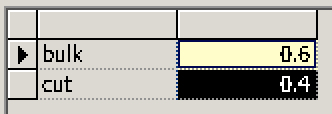
\includegraphics[width=0.33\textwidth]{./images/nodes/definitions/1.png}
\end{figure}
Usually people that do weightlifting want to build muscle. 
\item weight
\begin{figure}[H]
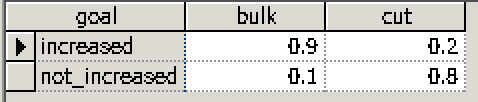
\includegraphics[width=0.66\textwidth]{./images/nodes/definitions/2.png}
\end{figure}
Of course, if we bulk we expect in almost all cases to increase our weight. Sometimes, due to some other factors, like stress or bad habits, this may influence our way to eat, train etx and thus we are not gain new weight. 

If the cut period is not properly planned, some people can eat a lot after a too strong diet and thus exponentially increase their weight instead of reduce it.

\item diet
\begin{figure}[H]
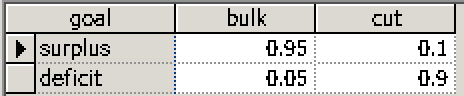
\includegraphics[width=0.66\textwidth]{./images/nodes/definitions/3.png}
\end{figure}

If we bulk we have no eat more, since this is very easy  we have a very low probably to still be in deficit. This reflect the case where we think we are eating enough but we are still in deficit. Cutting is harder since an athlete needs to correctly tracks is kcal so we have a 10\% probability of still beeing in surplus.

\item sleep
\begin{figure}[H]
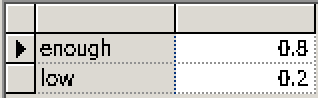
\includegraphics[width=0.33\textwidth]{./images/nodes/definitions/4.png}
\end{figure}

Some people does not sleep enough. Be aware that sleep does not only take in account the number of hours slept but also the time we go to bed. There is a big difference between an athlete that goes to bed at 23 and wakes up at 7 than one that goes to bed ad 01 and wakes up at 9.

\item rest
\begin{figure}[H]
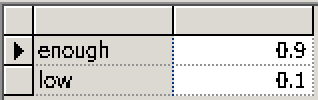
\includegraphics[width=0.33\textwidth]{./images/nodes/definitions/5.png}
\end{figure}

Even if is well know that our body need some rest time between workouts, some people still over train.

\item sex
\begin{figure}[H]
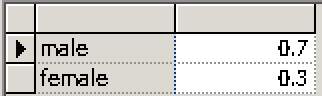
\includegraphics[width=0.33\textwidth]{./images/nodes/definitions/6.png}
\end{figure}
Most of the weightlifters are male.

\item genetic
\begin{figure}[H]
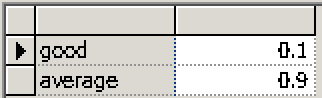
\includegraphics[width=0.33\textwidth]{./images/nodes/definitions/7.png}
\end{figure}
Only a small part of the population has a good genetic

\item body fat
\begin{figure}[H]
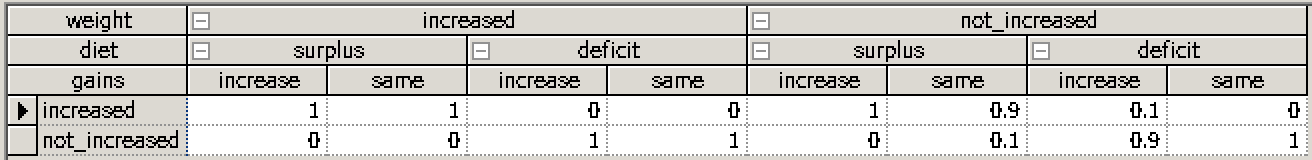
\includegraphics[width=\textwidth]{./images/nodes/definitions/8.png}
\end{figure}
Body fat depends on weight, diet and gains. If we are in surplus then our body fat will increase no matters what.

\item gains
\begin{figure}[H]
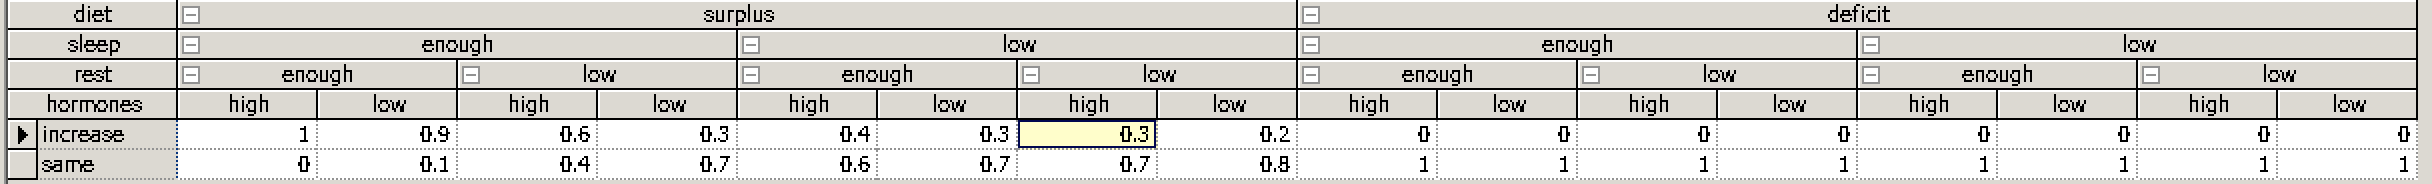
\includegraphics[width=\textwidth]{./images/nodes/definitions/9.png}
\end{figure}
Gains are the core node in the graph. They depends on a lot of factor. Intuitivelly, in everything goes well, first column, we will gain muscle. If some of the variables such as rest, sleep and diet are not positive we will probably not gain a lot

\item hormones
\begin{figure}[H]
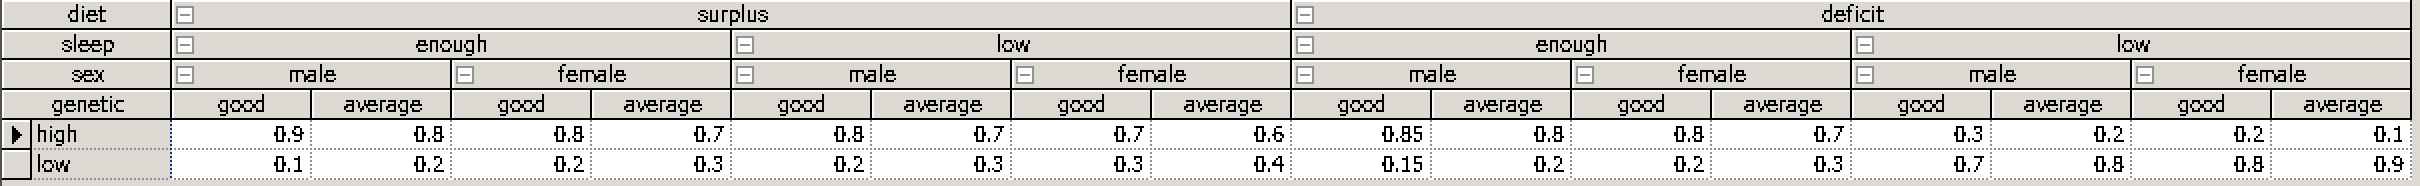
\includegraphics[width=\textwidth]{./images/nodes/definitions/10.png}
In our graph, hormones depends on diet, sleep, sex and genetic. With a diet in surplus, enough sleep we see a higher hormones in the population. If we also have a good genetic this value increases. Females have a slightly lower hormone productions than mans. On the other hand, if we don't sleep enough our body won't produce as much hormones as if we slept enough, this is reflected on the lower probabilities on having an hormone's high production showed in the table.
\end{figure}
\item 1RM 
\begin{figure}[H]
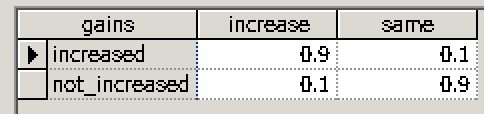
\includegraphics[width=0.5\textwidth]{./images/nodes/definitions/11.png}
\end{figure}
\end{itemize}

\section{Causal Inference}
I used the control value feature from genie (\texttt{https://support.bayesfusion.com/docs/GeNIe/bn\_controllingvalues.html}).
\subsection{Calculate the causal effect of X on Y.}
	I pick $X$ equal to \emph{diet} and $Y$ equal to \emph{body fat}. $X$ can assume two values, $deficit$ and $surplus$, while $Y$ can be $increased$ and $not\_increased$. We first want to find out
	\begin{equation}
		P(Y=y \given do(X=x))
	\label{eq:1}
	\end{equation}
	
We want to observe $Y$, so by plugging the values into \ref{eq:1}, we want to calculate
$P(Y=increased \given do(X=surplus))$ and $P(Y=increased \given do(X=deficit))$. We can easily do so with genie by controlling the value of $X$.

\begin{figure}[H]
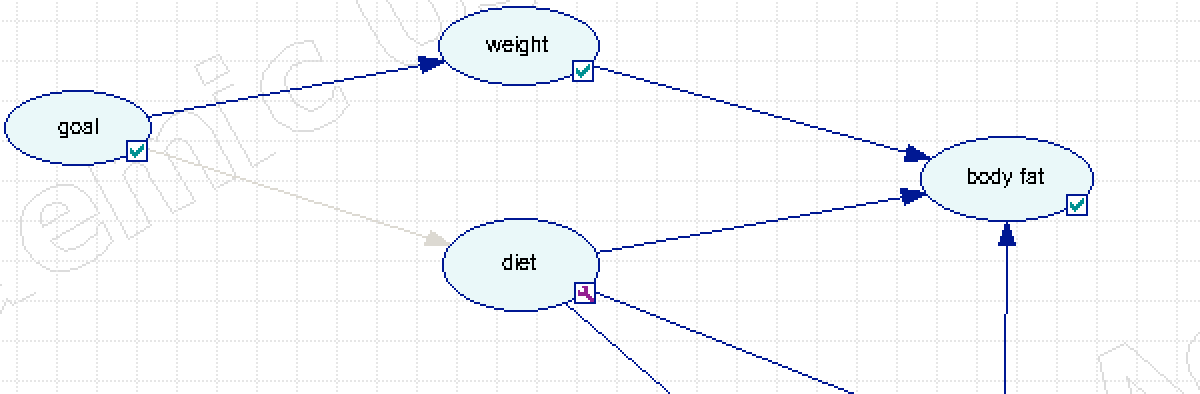
\includegraphics[width=\textwidth]{images/control_value/1}
\end{figure}

We obtain:
\begin{align}
P(Y=increased \given do(X=surplus)) = 0.993 \\
P(Y=not\_increased \given do(X=surplus)) = 0.007
\end{align}

The results make sense, since if we eat more than our baseline, $X=surplus$, we have an almost certain probability to weight more than last month. On the other hand, if we eat less than our baseline we are almost sure we can't increase our weight.

\subsection{Identify possible confounders between X and Y.}
There is no confounder between $X$ and $Y$
\subsection{Would it be practically possible in your specific problem to perform also a randomized controlled study to disentangle the causal effect between the variables from their correlation?
}
Yes, sure. In my problem perform a randomized controlled study is possible. The diet can be imposed to two groups of the population and then we can observe the effect on body fat.

\subsection{Compute the ACE of X on Y}
Average Causal Effect (ACE) is defined as follow:
\begin{equation}
P(Y=1 \given do(X=1)) - P(Y=1 \given do(X=0)) 
\label{eq: ace}
\end{equation}
Using Equation \ref{eq: ace} in our network

\begin{align}
&P(Y=increased \given do(X=surplus)) = 0.993 \\
&P(Y=increased\given do(X=deficit)) = 0
\end{align}
Thus
\begin{align*}
P(Y=increased \given do(X=surplus)) - P(Y=increased\given do(X=deficit)) = \\
=  0.993 - 0 = 0.993
\end{align*}
The ACE is $0.993$
\subsection{Choose another variable C and calculate the c-specific effect of X on Y.}
I choose $C$ to be goal, to calculate the c-specific effect. I want to calculate $P(Y=increase \given do(X=surplus), C=bulk)$. So the probability to gain fat given that we eat enough and we are in a bulking phase. Following rule 2 from the book, we also need the set of variables that blocks all the backdoor paths from $X$ to $Y$, in our case $C$ already blocks all the such paths.
\begin{align*}
&P(Y=increased \given do(X=surplus), C=bulk) &= \\
& P(Y=increased \given X=surplus, S=increase, Z=bulk)P(S=increase) &+  \\
& P(Y=increased \given X=surplus, S=same, Z=bulk)P(S=same) &= \\ 
& 1 \cdot 0.499 + 0.99 \cdot 0.501 &= 0.994 
\end{align*}
The results makes perfect sense since we want to find out the probability of gain weight if we eat more than the baseline and we are in a bulking phase.

\subsection{Identify a minimal set of variables that must be measured in order to estimate the c-specific effect of X on Y.}
In this case, $C$, $X$ and $Y$ since we have not any set $S$ of variable that we need to ensure the paths from $X$ to $Y$ are closed.

\subsection{Choose a function g and compute the effect of the conditional intervention of X=g(C) on Y}
Let $g(x) = 
\begin{cases} 
1 \quad if \ x = 1 \\
0 \quad if \ x =  0 
\end{cases}
$
So, using Equation 3.17 from the book:

\begin{align*}
P (Y = increase \given do(X=g(C)) &=  P(Y=increase \given do(X=surplus),C=bulk)P(C=bulk) \\
&+ P(Y= increase \given do(X=deficit),C=0)P(C=cut)
\end{align*}
From the previous point, we know that $P(Y=increase \given do(X=surplus),C=bulk) =   $

\end{document}
